\documentclass[../TDE1-E2.tex]{subfiles}%

\begin{document}
\section[s]"1"{Mesures de tensions et intensités}

  \QR{%
      Dans les circuits ci-dessous, quelles sont les valeurs affichées par les
  instruments de mesure si ceux-ci sont parfaits~? On donne : $E = \SI{5,0}{V}$ ;
  $r_1 = \SI{10}{\Omega}$ ; $R = \SI{20}{\Omega}$ ; $R_1 = \SI{30}{\Omega}$ ; $R_2
    = \SI{40}{\Omega}$. On rappelle que dans un circuit, les ampèremètres parfaits
  sont équivalents à des fils alors que les voltmètres parfaits sont équivalents à
  des interrupteurs ouverts.
  \begin{tcn}[sidebyside, blankest](null){}
    \begin{center}
        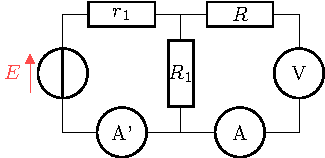
\includegraphics[width=\linewidth]{mes_iu_a-plain}
    \end{center}
    \tcblower
    \begin{center}
  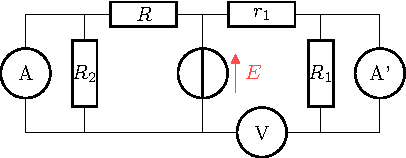
\includegraphics[width=\linewidth]{mes_iu_b-plain}
    \end{center}
  \end{tcn}
}{%
  \vspace{-15pt}
\begin{tcbraster}[raster columns=2, raster equal height=rows]
    \begin{tcn}(tool){Rappel}
        \begin{center}
            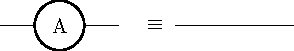
\includegraphics{amp_parfait}
            \smallbreak
            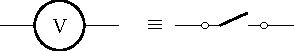
\includegraphics{volt_parfait}
        \end{center}
    \end{tcn}
    \begin{tcn}[sidebyside](data)'r'{Données}
        \begin{itemize}
            \item $E   = \SI{5.0}{V}$
            \item $r_1 = \SI{10}{\ohm}$
            \item $R   = \SI{20}{\ohm}$
        \end{itemize}
        \tcblower
        \begin{itemize}
            \item $R_1 = \SI{30}{\ohm}$
            \item $R_2 = \SI{40}{\ohm}$
        \end{itemize}
    \end{tcn}
\end{tcbraster}
\subsection{Schéma 1}
\begin{tcbraster}[raster columns=3, raster equal height=rows]
    \begin{tcn}(data){Schéma}
        \begin{center}
            \hspace*{-12pt}
            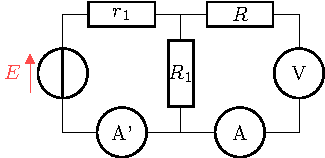
\includegraphics{mes_iu_a}
        \end{center}
    \end{tcn}
    \begin{tcn}(impl)""{Simplification}
        \begin{center}
            \hspace*{-12pt}
            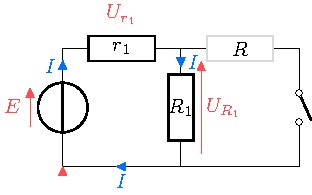
\includegraphics{mes_iu_a-simple}
        \end{center}
    \end{tcn}
    \begin{tcn}(appl)'r'{Application}

        V ouvre le circuit, donc aucun courant ne passe dans la boucle de
        droite~: A mesure \SI{0}{A}. On trouve $I$ avec la loi des mailles et on
        trouve $\DS I = \frac{E}{r_1 + R_1}$, et donc A' mesure \SI{0.125}{A}.
        Pour V, $R$ n'a pas de différence de potentiel donc il mesure $U_{R_1}
        = \SI{3.75}{V}$.

    \end{tcn}
\end{tcbraster}
\subsection{Schéma 2}
\begin{tcbraster}[raster columns=2, raster equal height=rows]
    \begin{tcn}(data){Schéma}
        \begin{center}
            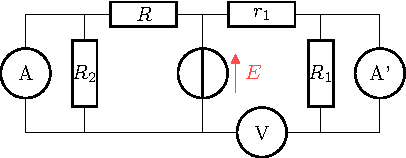
\includegraphics{mes_iu_b}
        \end{center}
    \end{tcn}
    \begin{tcn}*(impl)"limp"'r'{Simplification}
        \begin{center}
           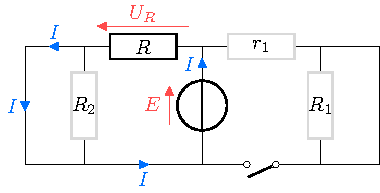
\includegraphics{mes_iu_b-simple}
        \end{center} 
    \end{tcn}
\end{tcbraster}
\begin{center}
    \begin{tcn}[width=\linewidth](appl){Application}
        Cette fois c'est la partie de droite qui est ouverte, et donc pas
        parcourue par un courant~: A' mesure \SI{0}{A}. L'ampèremètre de gauche
        court-circuite quant à lui la résitance $R_2$, ainsi toute l'intensité
        se trouve dans la boucle où on a tracé \textcolor{brandeisblue}{$I$}~;
        une rapide loi des mailles donne $\DS I = \frac{E}{R} = \SI{0.25}{A}$. V
        mesure ici aussi la tension $E$.
    \end{tcn}
\end{center}
}

\end{document}
